\section{Experimental Setup}
\label{sec:setup}

\begin{figure}[t]
    \centering
    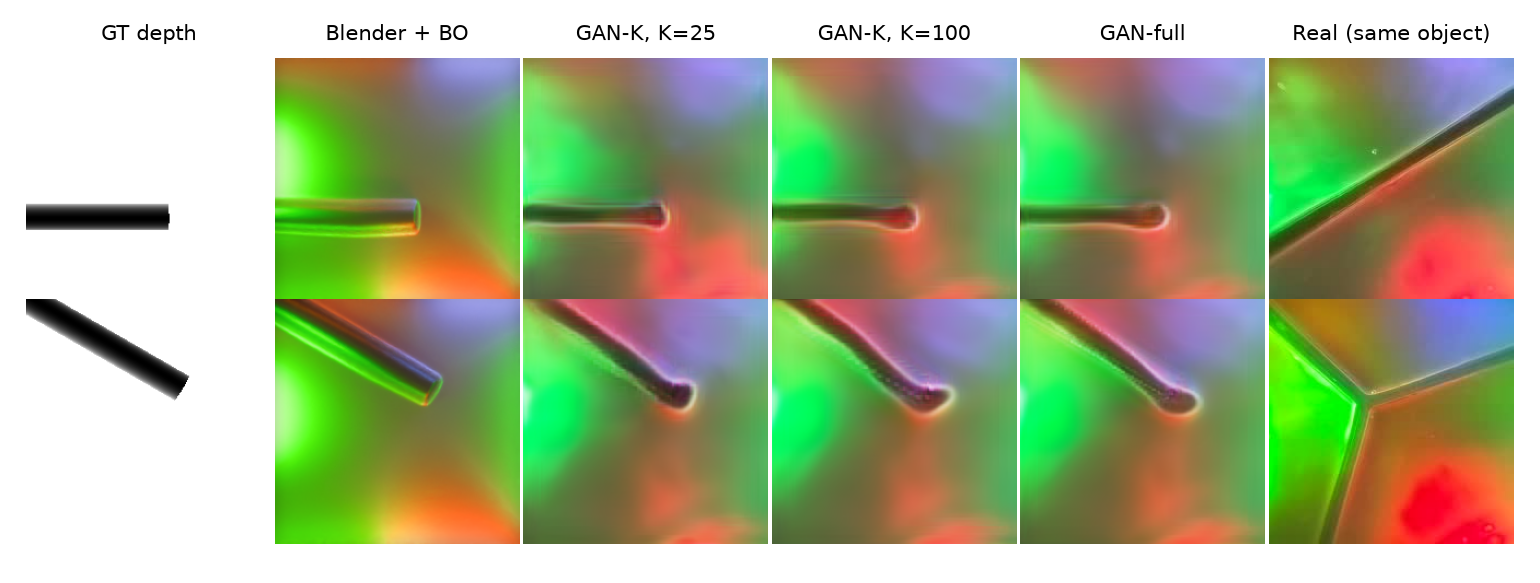
\includegraphics[width=\columnwidth]{figures/long/fig_renders.png}
    \caption{\textbf{Two renderers, one contact.} Each row is one simulated contact (GT depth, left) rendered by the physically calibrated Blender renderer, by the learned renderer trained on $\Kreal=25$ or $\Kreal=100$ real pairs per object, and by the learned renderer trained on all real pairs (GAN-full). Right: a real frame of the same object. PBR reproduces the illumination field but not the dark contact shading of the real gel; the learned renderers reproduce the shading and inherit the illumination of their training frames.}
    \label{fig:renders}
\end{figure}

\subsection{Sensors and Data}
\noindent\textbf{Sensor A.} Sensor A is GelSlim~5.0~\cite{wang2026gelslim}, a marker-free design with a $17.5\,$mm square gel view imaged under six colored LED emitters. Images are center-cropped to $0.816$ of the view and resized to $224\times224$.

\noindent\textbf{Real data (session 1).} A KUKA LBR Med arm presses the sensor onto 12 objects of known geometry, recording the image and end-effector pose at every contact; ground-truth (GT) depth and normals are the mesh projected at the recorded pose (geometric targets, not membrane measurements). After removing frames whose image contact region disagrees with the GT, $4{,}669$ frames remain ($222$--$568$ per object), one session per object, every tenth frame held out as validation ($472$ frames).

\noindent\textbf{Real data (session 2).} The same objects were re-placed and re-captured on another day (48 runs). GT poses were re-estimated per frame by maximizing the IoU between the image ridge mask and the projected mesh contact and manually reviewed; the curated test set has $854$ frames of $11$ objects (Sec.~\ref{sec:cross}). The session-1 calibration no longer held after re-placement (per-run corrections averaged $11^\circ$ and $1.6\,$mm). Apart from the label-free adaptation study of Sec.~\ref{sec:cross}, which trains on images from half of the session-2 presses without their poses and tests on the other half, nothing from this session is used for training or model selection.

\noindent\textbf{Sensor B.} Sensor B is GelSlim~4.0~\cite{sipos2024gelslim4}, with a marker array, a different illumination layout and a $12\,$mm field of view. Its public depth dataset~\cite{sipos2024gelslim4} has the same 12 objects pressed by a parallel gripper at $1\,$mm indentation with mesh-derived depth and in-hand pose labels ($135$ test frames per object). We use the left finger, the central $12\times12\,$mm, and report rotation after removing a per-object constant offset because its pose origin differs from ours.

The public depth labels are clipped at the nominal indentation and smoothed, so they are not exact mesh projections. For the AlignTac comparisons in Sec.~\ref{sec:sensorb}, a global search fits the planar mesh pose to each public label ($0.018\,$mm mean residual). We canonicalize the fitted pose using the object's rotational symmetry and use its projected mesh depth for training and testing (\emph{mesh-fitted} labels). A separate set of renderer experiments in Sec.~\ref{sec:sensorb} retains the original public labels; those results are identified explicitly.

\noindent\textbf{Contact sampler.} For each object we sample contact cells over the mesh at 12 base rotations ($30^\circ$ apart), an indentation of $0.8$--$1.2\,$mm and in-plane jitter, and export $D$ from the object z-buffer and $N$ by finite differences. Simulated poses are restricted to each object's real rotation and translation ranges. The same $5{,}345$ simulated contacts feed every renderer.

\subsection{Physically Calibrated Renderer}
\label{sec:blender}
The physically based renderer (PBR) is implemented in Blender/Cycles: a gel surface mesh is shrink-wrapped onto the object and smoothed (35 corrective iterations), shaded with a glossy/transparent material and a height-driven contact-darkening term, lit by six area emitters, and post-processed (saturation, brightness, contrast, haze, a low-frequency random gel warp). Emitter and post-processing parameters (16 scalars) are fitted by tree-based Bayesian optimization of an $L_2$ plus histogram distance between the real and rendered no-contact image (500 evaluations); gel and contact parameters were hand-tuned by visual comparison with a single separately captured calibration contact of one object, which is not among the held-out objects. Thus, the renderer sees one no-contact image and one contact image, without depth or pose labels; neither is counted in the label budget.

\noindent\textbf{Domain-randomization baseline.} To test whether careful calibration is necessary, we also render with randomized sensor parameters: random HSV colors and strengths for each LED emitter, random gel optics, per session, with the geometry stage (scale, field of view, smoothness) fixed. This variant uses no image to fit its randomized appearance parameters; it retains the shared geometry configuration.

\subsection{Learned Renderer}
\label{sec:gan}
The learned renderer is a conditional GAN~\cite{isola2017pix2pix}: a five-level U-Net that takes the depth map and two coordinate channels and outputs an RGB image, a $70\times70$ spectral-normalized PatchGAN discriminator, and an adversarial $+\,100\,(\mathrm{L1} + \mathrm{gradient\;L1} + \mathrm{low\text{-}frequency\;L1})$ loss. Simulated depth is jittered by $\pm15\%$ at generation time.

\noindent\textbf{Real budget.} GAN-$\Kreal$ is trained on $\Kreal$ real (depth, image) pairs per object, an evenly spaced subset of each object's training frames that is \emph{the same} $\Kreal$ frames the downstream model receives; GAN-LOO on all training frames of the 9 non-held-out objects; GAN-full on all $4{,}197$ pairs in the legacy protocol, or on the $3{,}667$ pairs that exclude the held-out test frames in the clean protocol. Small budgets train for at least $30$k generator updates.

\noindent\textbf{Variants.} \emph{Background-conditioned}: the session's no-contact image is appended as three input channels, providing session illumination from one background frame. \emph{Physics-conditioned}: PBR's image of the same contact is appended, optionally predicting only a residual on top of it, optionally with the background. \emph{Difference image}: the target is the image minus the session background. \emph{Blender-pretrained}: pretraining on $30$k (depth, Blender image) pairs, then fine-tuning on the real pairs.

\emph{Multi-sensor}: the background-conditioned GAN is trained on 100 simulated sensor designs (random LED layouts and gel materials) plus optionally the target sensor's real pairs; this tests whether sensor diversity can replace sensor-specific real data. \emph{Rotation coverage} changes the geometry stage instead: we vary how many of an object's real rotations appear in simulation (1, 2 or all 12) and, for the learned renderer, rotate the depth map before rendering so that every rotation is covered.

\subsection{Zero-Label Alternative: Contact-Preserving Unpaired Refiner}
\label{sec:refiner}
We also test whether unlabeled real images can improve synthetic appearance without paired renderer supervision. Following unpaired image translation~\cite{shrivastava2017simgan,park2020cut,chen2022cyclegan}, we train a refiner to change the shading of a physical render while preserving its contact region. The refiner $\mathcal{F}$ takes the physical render $\hat{\mathcal{I}}_{\mathrm{phys}}$, the session background $B$ and the contact mask $m$ (simulated depth $>0$, dilated by 4\,px and feathered) and outputs
\begin{equation}
    \hat{\mathcal{I}} = m \odot \mathcal{F}(\hat{\mathcal{I}}_{\mathrm{phys}}, B, m) + (1-m) \odot B ,
\end{equation}
The background is therefore taken from the real sensor, while the refiner changes only the contact region. Depth, normal and pose targets remain those of the physical render.

 $\mathcal{F}$ is the same U-Net as the learned renderer with a 7-channel input. It is trained against a $70\times70$ PatchGAN on \emph{unlabeled} real frames (image only; no depth, no pose) with an adversarial loss and a patchwise contrastive loss (PatchNCE~\cite{park2020cut}) between the encoder features of input and output, sampled preferentially inside $m$, to encourage preservation of the rendered ridge structure. We train for 10k generator updates with batch size 8 and Adam ($2\times10^{-4}$, $\beta_1=0.5$).

Its real budget is the set of unlabeled frames plus one background frame per session, and the same leakage rule applies: in leave-object-out the held-out objects' frames are excluded, in $\Kreal$-shot the same $\Kreal$ frames as the downstream model are used without their labels. With domain-randomized inputs, the refiner requires no appearance calibration or paired training labels; it retains the shared geometry configuration.

\subsection{Downstream Tactile Model}
The downstream model is identical for every renderer: a frozen sensor-invariant encoder (SITR-B/18~\cite{gupta2025sitr}) provides patch tokens at four depths; a DPT decoder~\cite{ranftl2021dpt} predicts depth and normals at $224\times224$; a pose head regresses $(\cos\theta,\sin\theta,t_x,t_y)$ from the class token and mean patch token. For the classification study, we add a 12-class head (LayerNorm on concatenated class and mean patch tokens, two-layer MLP with GELU) and train with cross-entropy alongside the other losses. The decoder, pose head and object embedding are trained ($12$M parameters). Losses are MSE on depth and normals, $1-\cos(\theta-\hat\theta)$ on rotation and L1 on translation, balanced by grouped uncertainty weighting~\cite{kendall2018multi}.

When synthetic data is used, training mixes simulated and real frames. Simulated frames receive photometric augmentation and $\pm15^\circ$ gel-spin rotation with matched labels; real frames are not augmented. We use AdamW with learning rate $2\times10^{-4}$, batch size 32 and a cosine schedule. Main sensor-A runs use 150 epochs, while sensor B and seed/ablation studies use 50. Depth and normal metrics use the checkpoint with the lowest validation depth MSE (at $K\le25$ within the first ten epochs). Pose metrics use the checkpoint with the lowest validation rotation error in every table and figure, including the session-2, sensor-B and test-time refinement evaluations; the pose head does not overfit (final-epoch and selected-epoch rotation agree within $0.3^\circ$), whereas rotation at the early dense checkpoint mainly reflects its short training. Translation error is the mean absolute error over the two coordinates. In every case, checkpoint selection uses validation labels in addition to the $K$ training labels.

\subsection{AlignTac Implementation}
Aligner perturbations span $\pm8^\circ$, $\pm1.5\,$mm in-plane and $\pm0.15\,$mm in indentation; half use ranges scaled by $0.3$. Training uses smooth L1 for 8,000 steps (batch 64, AdamW, learning rate $3\times10^{-4}$). Aligners train on real examples only, the teacher uses the $K$ real frames, and the student receives no synthetic frame. The \emph{+ learned synth.} variant (sensor A) mixes 24 real and 40 synthetic examples generated by the $K$-pair renderer in each aligner batch, trains the teacher with learned-renderer data, and gives the student synthetic images from a renderer retrained on labeled and aligned real pairs.

On one RTX 6000 Ada GPU, aligner training takes about $20$ minutes, labeling $0.5\,$s per frame ($30$ minutes for the $3{,}897$ sensor-A frames), and student training $1.3$ hours for 50 epochs or $2.2$ hours for 150. The renderer, when used, adds about one hour.

\subsection{Data-Access Protocol}
\label{sec:protocol}
Paired renderers and the aligner exclude validation and test images from training. The $K$-shot protocol additionally limits paired training labels to the same $K$ frames per object. Validation labels remain available for model selection; the reported budget counts training labels. Physical-renderer manual tuning is described separately above.

\noindent\textbf{Two evaluation protocols.} The headline sensor-A results (Table~\ref{tab:kshotT}, Table~\ref{tab:rcablT}, the test-time alignment table and Figs.~\ref{fig:kshot}, \ref{fig:conv} and \ref{fig:qual}) follow a clean protocol: $530$ session-1 frames (every tenth and every eighth-of-ten frame that is not among the $K$ labeled contacts) are held out from all training, including renderer fitting and pseudo-labeling, and every number is reported on them; the $472$ validation frames are used only for checkpoint selection. The extended variant tables (Tables~\ref{tab:kshot}--\ref{tab:rcabl}, \ref{tab:cross}, \ref{tab:selection} and \ref{tab:variants}) predate this split and report the legacy protocol, in which models were selected and evaluated on the same validation frames; they are kept for the additional variants they cover and are marked as such. Under both protocols the conclusions are identical.

\noindent\textbf{Leave-object-out (LOO).} Three objects (a two-line, a rod and a cross pattern; $1{,}244$ frames) are removed from all real training, excluded from paired-renderer and aligner training, and evaluated in full. Simulated contacts of the three meshes are available to every renderer (``new object with a CAD model but no real touches''). A \emph{geometry control} additionally removes the three meshes from simulation.

\noindent\textbf{$\Kreal$-shot.} Every object contributes $\Kreal\in\{0,10,25,50,100\}$ evenly spaced real training frames. For $K>0$, the learned renderer is trained on exactly those frames; the downstream model co-trains on them plus simulated data, or on them alone with the same number of updates. Evaluation is on the real validation split. The aligner of AlignTac receives the same $\Kreal$ frames, and the remaining training frames may be used \emph{without} their labels.

\noindent\textbf{Cross-session and cross-sensor.} Session-2 and sensor-B test frames are never used to train or select anything in the sensor-A study. In the sensor-B study the $\Kreal$-shot protocol is repeated with sensor-B real pairs and the sensor-B test split.

\noindent\textbf{Learned renderer (full).} GAN-full is trained on all sensor-A training pairs ($4{,}197$ in the legacy protocol; $3{,}667$ in the clean protocol, which excludes the held-out test frames). In LOO, these include real pairs from held-out objects; in $K$-shot, they include training labels withheld from budget-matched methods, but no validation frames. We label this non-comparable reference ``learned renderer (full)''; it is shown in italics and excluded from best-result highlighting.

\noindent\textbf{Metrics.} We report depth MSE over all pixels ($\mathrm{mm}^2$), following prior work on this sensor. Because $\approx90\%$ of pixels are background, we also report mean absolute error inside the GT contact region (contact MAE, mm) and contact IoU (predicted depth $>0.05\,$mm vs.\ GT $>0$), which also penalizes false contact. Normals are evaluated by mean angular error inside the contact region (deg), and pose by mean rotation error (deg) and translation error (mm; mean absolute error over the two coordinates).
